
\section{Search and Planning Foundations}
\label{sec:single-agent-search}
\hspace{\parindent}
Classical graph search techniques provide an important foundation for MRPP and MAPF methods,
since they are commonly used to compute individual robot paths and to support coordination
strategies. In the context of this dissertation, these methods are particularly relevant because the
considered fleet coordination framework performs planning over a graph representation of the
environment.

Accordingly, this section reviews graph search and planning concepts that underlie the TEA*
planner used in this work and many related multi-robot coordination approaches. The focus is first
placed on shortest path search in graphs and then on heuristic search, with particular emphasis on
Dijkstra's algorithm and A*.



\subsection{Search Problems on Graphs}
\hspace{\parindent}
A search problem on a graph consists of finding a sequence of transitions that leads from a
given initial state to a goal state while satisfying feasibility constraints and optimizing a
specified cost criterion \cite{russell2010aima}.

Formally, a search problem is defined by a state space, an initial state, a set of goal states,
a transition model that specifies the allowable moves between states, and a cost function that
assigns a non-negative cost to each transition or path \cite{russell2010aima}. When the state
space is represented explicitly as a graph, vertices correspond to states and edges encode
feasible transitions, possibly associated with traversal costs.

A solution to a graph search problem is a path in the graph that connects the initial vertex
to a goal vertex. Among all feasible solutions, particular interest is often placed on optimal
solutions, defined as those that minimize the cumulative cost along the path. The shortest path
problem in weighted graphs is a canonical instance of this formulation and has been extensively
studied in both theoretical and applied contexts \cite{cormen2009introduction}.

Search algorithms typically operate by incrementally exploring the graph starting from the
initial state, expanding states according to a specific strategy and maintaining a frontier of
candidate paths. Different search strategies define different orders in which states are
expanded, which directly affects properties such as completeness, optimality, and computational
efficiency \cite{hart1968formal}.

\subsubsection{Dijkstra's Algorithm}
\hspace{\parindent}
Dijkstra's algorithm is a classical graph search algorithm for solving the shortest path problem
in weighted graphs with non-negative edge costs. Originally introduced by Dijkstra
\cite{dijkstra1959note}, it provides a systematic procedure for computing the minimum-cost path
from a given initial vertex to all other reachable vertices in the graph.

The algorithm operates by incrementally expanding vertices in order of increasing accumulated
path cost from the initial state. At each step, the vertex with the lowest known cost is selected
for expansion, and its outgoing edges are relaxed to update the cost of reaching neighboring
vertices. This process continues until the goal vertex is reached or all reachable vertices have
been explored \cite{cormen2009introduction}.
A key property of Dijkstra's algorithm is that, under the assumption of non-negative edge costs,
once a vertex is expanded, the cost associated with it is guaranteed to be optimal. As a result,
the algorithm is both complete and optimal for this class of graphs \cite{cormen2009introduction}.

From a search perspective, Dijkstra's algorithm can be viewed as a best-first search strategy in
which the expansion order is determined by the accumulated path cost from the initial
vertex. This accumulated cost, commonly denoted by $g(n)$ for a vertex $n$, corresponds to the
sum of the costs of the edges along the path from the initial vertex to $n$
\begin{equation}
\label{eq:gn}
g(n) = \sum_{(u,v) \in P_n} c(u,v),
\end{equation}
where $P_n$ denotes the path to $n$ and $c(u,v)$ is the cost of edge from vertex $u$ to vertex $v$.


Regarding computational complexity, the cost of Dijkstra's algorithm depends on the data structure used to manage the frontier. When implemented with a binary heap priority queue and an adjacency-list graph representation, the algorithm has worst-case time complexity

\begin{equation}
\label{eq:dijkstra_complexity}
    O\bigl((|V| + |E|)\log |V|\bigr),
\end{equation}
where \(|V|\) is the number of vertices and \(|E|\) is the number of edges in the graph \cite{cormen2009introduction}. This bound results from inserting and updating vertices in the priority queue while relaxing the graph edges.

 In MRPP settings, it is often used as a baseline within more complex coordination frameworks, serving as a
reference point for evaluating the benefits more advanced search
strategies.



\subsubsection{A* Search Algorithm}
\label{subsubsec:astar_search_algorithm}
\hspace{\parindent}
A* is a heuristic-based graph search algorithm that extends Dijkstra’s algorithm by
incorporating problem-specific information to guide the search toward the goal more efficiently.
Originally introduced by Hart, Nilsson, and Raphael \cite{hart1968formal}, A* is designed to
compute optimal paths while reducing the number of explored states when compared to uninformed
search methods.

The algorithm evaluates each vertex using an objective function
\begin{equation}
f(n) = g(n) + h(n),
\end{equation}
where $g(n)$ denotes the accumulated cost from the initial vertex to vertex $n$, as defined in
Equation~\eqref{eq:gn}, and $h(n)$ is a heuristic estimate of the remaining cost from $n$ to a
goal vertex.


This algorithm maintains a frontier of candidate vertices ordered by increasing values of 
$f(n)$ and iteratively expands the vertex with the lowest estimated total cost. When the heuristic
function is admissible, meaning that it never overestimates the true remaining cost to the
goal, A* is guaranteed to be both complete and optimal \cite{hart1968formal, pearl1984heuristics}. 

Figure~\ref{fig:dijkstra_vs_astar} illustrates the resulting difference in exploration behavior
between Dijkstra's algorithm and A*. The light blue marker denotes the initial state, the green
marker denotes the goal state, and darker blue cells correspond to expanded nodes. The
environment is modeled as a grid to facilitate visualization, and the Manhattan distance
heuristic is used to guide the A* search. As can be observed, in this particular example, the
heuristic effectively directs the search toward the goal, resulting in a focused expansion
pattern, whereas Dijkstra's algorithm exhibits a nearly radial expansion that explores the state
space more uniformly. However, this figure should be interpreted as an illustrative case rather
than as a general performance guarantee. The advantage of A* depends on the informativeness of
the heuristic function and on the structure of the search problem, with a weak or uninformative
heuristic, its exploration behavior may become much closer to that of Dijkstra's algorithm.





From a search perspective, Dijkstra's algorithm can be seen as a special case of A* in which
the heuristic function is identically zero. Under this interpretation, A* generalizes Dijkstra
by allowing heuristic guidance while preserving optimality guarantees under appropriate
conditions \cite{cormen2009introduction}.

The computational complexity of A* also depends on the implementation of the frontier and on the effectiveness of the heuristic function. In the worst case, when the heuristic provides no useful guidance, A* may explore the same search space as Dijkstra's algorithm. With a binary heap priority queue and an adjacency-list graph representation, its worst-case time complexity is therefore the same as in Equation~\ref{eq:dijkstra_complexity}.

In practice, an informative admissible heuristic can reduce the number of expanded vertices, but the worst-case bound remains the same.

\begin{figure}[H]
    \centering
    \begin{subfigure}{0.40\linewidth}
        \centering
        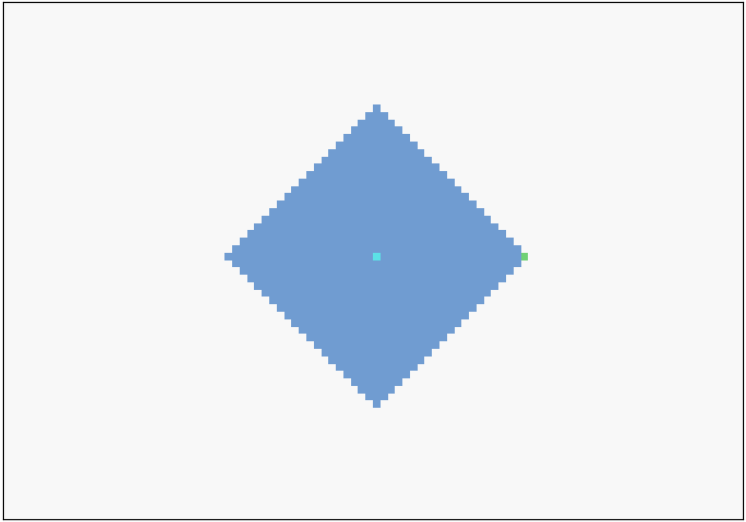
\includegraphics[width=\linewidth]{dijkstra_expansion.png}
        \caption{Dijkstra}
    \end{subfigure}
    \hspace{0.03\linewidth}
    \begin{subfigure}{0.40\linewidth}
        \centering
        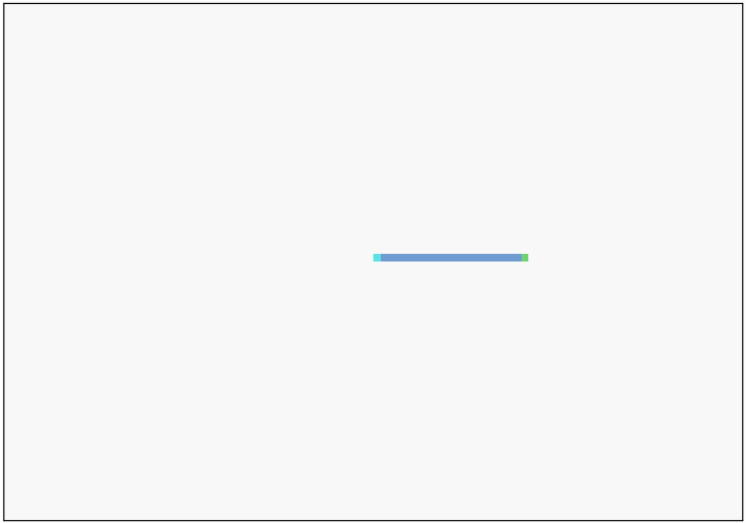
\includegraphics[width=\linewidth]{astar_expansion.png}
        \caption{A*}
    \end{subfigure}
    \caption{Comparison of node expansion patterns produced by Dijkstra's algorithm and A*.}
    \label{fig:dijkstra_vs_astar}
\end{figure}
